\documentclass{beamer}
\mode<presentation>
{
  \usetheme{Warsaw}
  \definecolor{mcgarnet}{rgb}{0.38, 0, 0.08}
  \definecolor{mcgray}{rgb}{0.6, 0.6, 0.6}
  \setbeamercolor{structure}{fg=mcgarnet,bg=mcgray}
  %\setbeamercovered{transparent}
}


\usepackage[english]{babel}
\usepackage[latin1]{inputenc}
\usepackage{times}
\usepackage[T1]{fontenc}
\usepackage{tikz}
\usepackage{graphicx}

\newcommand{\imagesource}[1]{{\centering\hfill\break\hbox{\scriptsize Image Source:\thinspace{\small\itshape #1}}\par}}

\title{Effective Object Oriented Design}


\author{Robert Lowe\\}

\institute[Maryville College] % (optional, but mostly needed)
{
  Division of Mathematics and Computer Science\\
  Maryville College
}

\date[]{}
\subject{}

\pgfdeclareimage[height=0.5cm]{university-logo}{images/Maryville-College}
\logo{\pgfuseimage{university-logo}}



\AtBeginSection[]
{
  \begin{frame}<beamer>{Outline}
    \tableofcontents[currentsection]
  \end{frame}
}


\begin{document}

\begin{frame}
  \titlepage
\end{frame}

\begin{frame}{Outline}
  \tableofcontents
\end{frame}


% Structuring a talk is a difficult task and the following structure
% may not be suitable. Here are some rules that apply for this
% solution: 

% - Exactly two or three sections (other than the summary).
% - At *most* three subsections per section.
% - Talk about 30s to 2min per frame. So there should be between about
%   15 and 30 frames, all told.

% - A conference audience is likely to know very little of what you
%   are going to talk about. So *simplify*!
% - In a 20min talk, getting the main ideas across is hard
%   enough. Leave out details, even if it means being less precise than
%   you think necessary.
% - If you omit details that are vital to the proof/implementation,
%   just say so once. Everybody will be happy with that.
\section{Software Engineering Overview}
\begin{frame}
    \frametitle{Software Development Lifecycle}
    \begin{columns}
    \column{0.6\textwidth}
    {\bf Stages of Software Development}
    \begin{enumerate}[<+->]
        \item Requirement Gathering and Analysis
        \item Design
        \item Implementation
        \item Testing
        \item Deployment
        \item Maintenance
    \end{enumerate}
    \begin{block}{Reality Check}<+->
        In the real world, the above is step 1.  The software then enters
        a cycle until it is decommissioned!
    \end{block}
    \column{0.4\textwidth}
    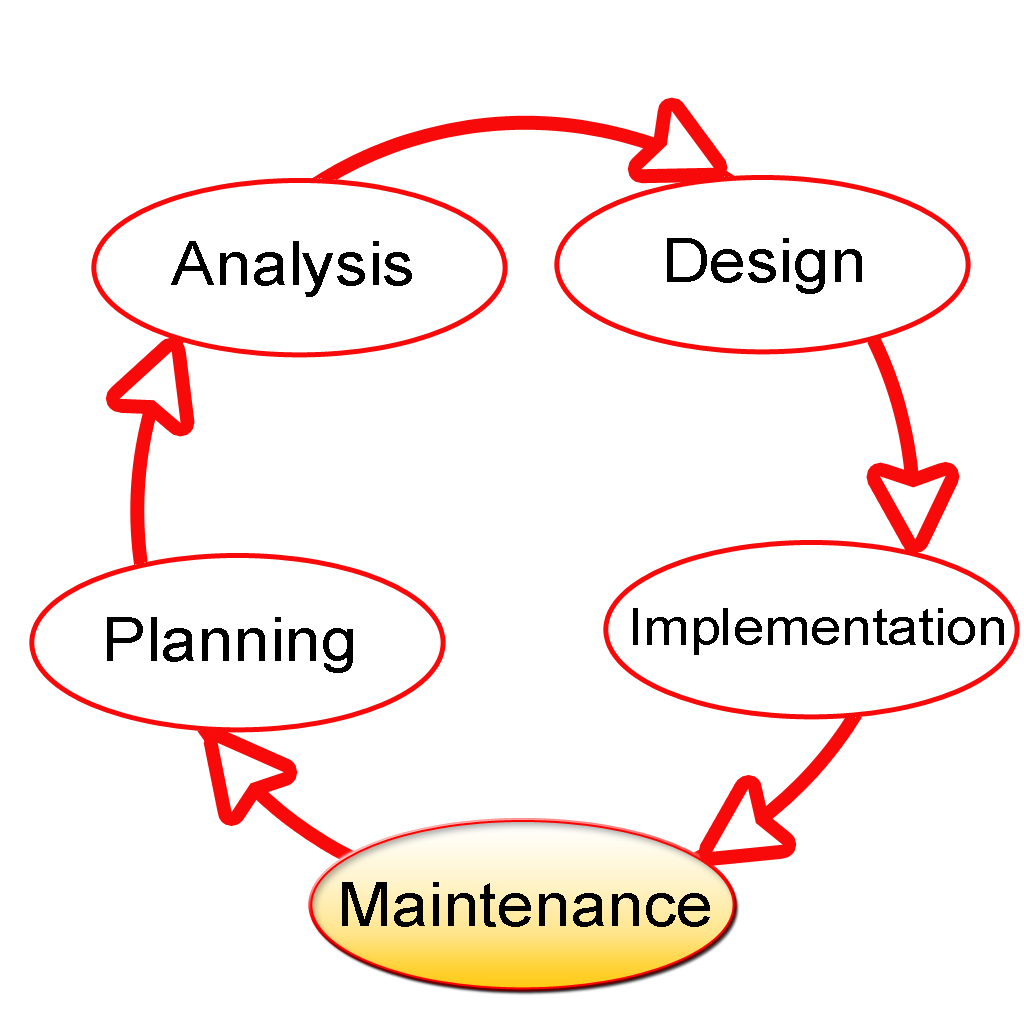
\includegraphics[width=\textwidth]{images/sdlc}
    \imagesource{wikipedia.org}
    \end{columns}
\end{frame}

\begin{frame}
    \frametitle{Software Engineering Overview}
    \begin{itemize}[<+->]
        \item Software engineering is any methodology by which requirements are gathered and software is designed.
        \item Communication is the primary concern.
        \item SE is also used to determine success or failure in a software project.
        \item SE also provides a methodology of managing development resources and time.
        \item There is no silver bullet that makes software easy to develop.
        \item Every year, someone attempts to promote a new "Silver Bullet".
        \item Ignore them.
    \end{itemize}
\end{frame}

\begin{frame}
    \frametitle{Communication with Stakeholders}
    \begin{columns}
        \column{0.6\textwidth}
        \begin{itemize}[<+->]
            \item A stakeholder is anyone involved with, or affected by, a project.
            \item Programmers
            \begin{itemize}[<+->]
                \item High Technical Knowledge
                \item Low Business Acumen 
                \item Often Not a Domain Expert
            \end{itemize}
            \item Managers and Clients
            \begin{itemize}[<+->]
                \item Low Technical Knowledge
                \item High Business Acumen
                \item Domain Experts
            \end{itemize}
            \item A big part of software engineering is putting these two worlds  together!
        \end{itemize}
        \column{0.4\textwidth}
        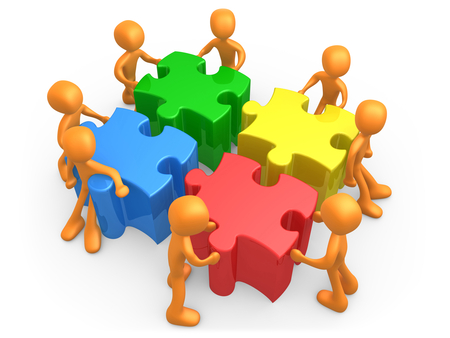
\includegraphics[width=\textwidth]{images/stakeholders}
    \end{columns}
\end{frame}

\begin{frame}
    \frametitle{Software Engineering Model: Waterfall}
    \begin{itemize}[<+->]
        \item The oldest software engineering method.
        \item It seems to make sense.
        \item It rarely works well.
        \item When it works, it works really well.
        \item When it fails, it is catastrophically expensive.
        \item Process of Propositions and Sign-offs
        \begin{enumerate}[<+->]
            \item Requirements
            \item Design 
            \item Implementation
            \item Verification
            \item Maintenance
        \end{enumerate}
    \end{itemize}
\end{frame}

\begin{frame}
    \frametitle{Agile Methodologies}
    \begin{itemize}[<+->]
        \item Waterfall is old and stodgy.  Agile is young and hep!
        \item Agile methodologies are cyclic.
        \item The focus is on early prototyping, with heavy stakeholder involvement.
        \item Development continues until everyone is happy (or so unhappy they
           terminate the project.)
        \item Examples of Agile Methodologies
        \begin{itemize}[<+->]
            \item Extreme Programming
            \item Crystal Clear Methods
            \item Feature Driven Development
            \item Adaptive Software Development
            \item Scrum
            \item Test-Driven Development
        \end{itemize}
        \item Most agile methodologies assume OOP, and maybe some functional
           programming.
    \end{itemize}
\end{frame}

\section{Object Oriented Analysis and Design}
\begin{frame}
    \frametitle{Object Oriented Analysis}
    \begin{itemize}[<+->]
        \item {\bf Goal: } Determine what the objects are and how they interact.
        \item {\bf Methodology}
        \begin{enumerate}[<+->]
            \item Gather requirements, get a basic understanding.
            \item Create use cases to analyze user interactions.
            \item Tease out objects by studying use cases.
            \item Sketch out how objects interact with each other.
            \item Create a rudimentary object/class layout.
        \end{enumerate}
    \end{itemize}
\end{frame}

\begin{frame}
    \frametitle{Object Oriented Design}
    \begin{itemize}[<+->]
        \item {\bf Goal:} Create a detailed technical design which fully 
            specifies classes, attributes, and methods.
        \item {\bf Methodology}
        \begin{enumerate}[<+->]
            \item Group objects together to identify classes.
            \item Use use cases and object descriptions to create attributes.
            \item Use object interactions and use cases to create object methods.
            \item Analyze classes, looking for commonalities.
            \item Establish abstract classes and inheritance relationships.
        \end{enumerate}
    \end{itemize}
\end{frame}

\begin{frame}
    \frametitle{Building Flexible Designs}
    \begin{itemize}[<+->]
        \item The real key to successful OOADP is to make flexible and reusable
            object.
        \item Design cohesive objects!  Each object should be a thing unto itself.
        \item Objects which do too much should likely be split apart.
        \item If it's not a noun, it's not an object!
        \item Create and abide by your object's method interfaces.
        \item Play by your own rules.  No object should be tightly coupled
            with non-public behavior of another object.
        \item Remember, agile implies changes, write general objects which can cope
            with change!
    \end{itemize}
\end{frame}

\section{Unified Modeling Language - UML}
\begin{frame}
    \frametitle{UML Overview}
    \begin{columns}
        \column{0.6\textwidth}
        \begin{itemize}[<+->]
            \item A graphical design language.
            \item Programming Language Agnostic.
            \item Comprised several types of diagrams.
            \begin{itemize}[<+->]
                \item Use Case Diagram
                \item Object Diagram
                \item Sequence Diagram
                \item Class Diagram
            \end{itemize}
            \item Used to Design, Communicate, and Clarify Software Systems
        \end{itemize}
        \column{0.4\textwidth}
        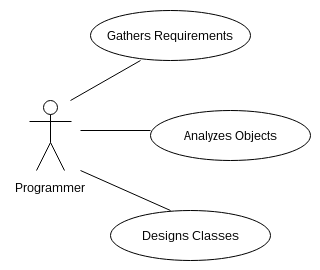
\includegraphics[width=\textwidth]{images/programmerUseCase}
    \end{columns}
\end{frame}

\begin{frame}
    \frametitle{Use Case Diagrams}
    \begin{columns}
    \column{0.6\textwidth}
    \begin{itemize}[<+->]
        \item A Use Case diagram outlines the ways in which a system will be used.
        \item Each class of actor performs a series of actions.
        \item Actors are represented as a stick figure.
        \item Performance of tasks is represented as a line.
        \item Often differentiates different types of users.
    \end{itemize}
    
    \column{0.4\textwidth}
    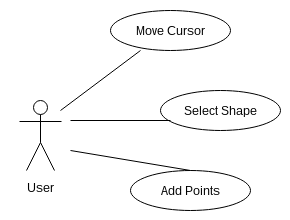
\includegraphics[width=\textwidth]{images/shapeUser}
    \end{columns}
\end{frame}

\begin{frame}
    \frametitle{Class Diagrams}
    \begin{columns}
    \column{0.5\textwidth}
    \begin{itemize}[<+->]
        \item A class diagram shows specification of the program's classes.
        \item Inheritance Relationships
        \item Class Attributes
        \item Class Methods
    \end{itemize}
    \column{0.5\textwidth}
    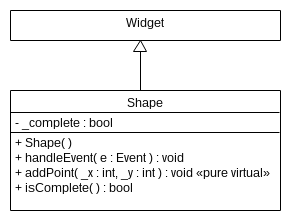
\includegraphics[width=\textwidth]{images/shapeClass}
    \end{columns}
\end{frame}

\begin{frame}
    \frametitle{UML for Object Oriented Analysis}
    \begin{itemize}[<+->]
        \item Analysis begins with conversations and study of the problem at hand.
        \item The first diagram, or set of diagrams, to draw is the Use Case diagram.
        \item Examine the use case diagram, review them with clients, and add/remove 
            use cases as needed.
        \item Use the use case diagram to draw a rudimentary class diagram, with 
            class names and relationships only.
    \end{itemize}
\end{frame}

\begin{frame}
    \frametitle{UML for Object Oriented Design}
    \begin{itemize}[<+->]
        \item Using your use case diagram, and your rudimentary class diagram,
            work out necessary methods and attributes for your classes.
        \item Add methods and attributes to your class diagram.
        \item Identify classes which should have super classes, and build 
            inheritance relationships.
        \item Split classes that don't make sense as cohesive objects.
        \item Keep building the class diagram until it fully models your program!
        \item Use the class diagram as a road map when you move on to implementation.
    \end{itemize}
\end{frame}

\begin{frame}
    \frametitle{Case Study: Object Oriented Pong}
    Let's perform OOAD on pong, using UML!
    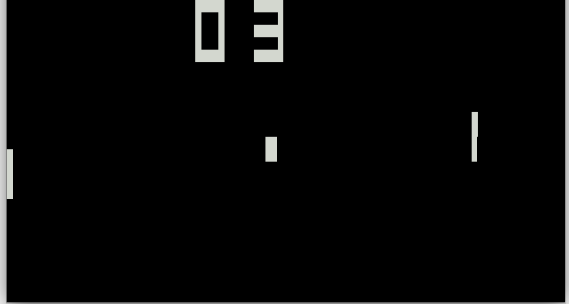
\includegraphics[width=\textwidth]{images/pong}
\end{frame}

\end{document}


